\chapter{Výsledky}
\section{Trénovanie dátových modelov}
Na začiatku sa náš systém nachádza v ustálenom stave, ktorý je definovaný optimálnou rýchlosťou riedenia nominálneho modelu $ D_N^{\star}=0.376\si{\per\hour} $. Údaje o koncentrácii substrátu a biomasy sme schopný zbierať každých 5 hodín po dobu 50 hodín (za tento čas sa systém dostane do ustáleného stavu po skokovej zmene). Na základe získaných dát zo zariadenia a nominálneho modelu vieme skonštruovať údaje o rozdieloch koncentrácie substrátu $ \Delta_{s} $ alebo biomasy $ \Delta_{x} $ a na týchto dátach môžeme identifikovať FIR alebo ARX model. Aby sme sa vyhli modelom zbytočne vysokého rádu, zvolili sme pri identifikácii metódou garantovaného odhadu parametrov chybu modelu rovnú dvojnásobku rozptylu šumu. 

V počiatočnom ustálenom stave by mal byť priebeh rozdielov koncentrácie biomasy aj substrátu konštantný, takže najjednoduchší FIR model, ktorý dokáže takéto dáta opísať je model prvého rádu a modely vyššieho rádu tým pádom neprichádzajú v úvahu. Výsledky identifikácie FIR modelov, ako aj ARX modelov, demonštrujeme na dátach v 3. iterácii optimalizačného procesu. Dôvodom je, že identifikácia modelu je kvalitnejšia pri väčšom počte údajov a v tomto bode sa objavila aj výraznejšia skoková zmena, v prípade údajov substrátu.

Zamerajme sa najskôr na hybridný model, ktorý koriguje hodnoty koncentrácie biomasy.  Výstupné údaje zo zariadenia a nominálneho modelu, môžeme vidieť na Obr. \ref{fig:FIR_bio_data} a podobne aj dáta rozdielov, ktoré sú zobrazené na Obr. \ref{fig:FIR_bio_ident}.
\begin{figure}
\centering
	\begin{subfigure}[b]{0.49\textwidth}
		\centering
		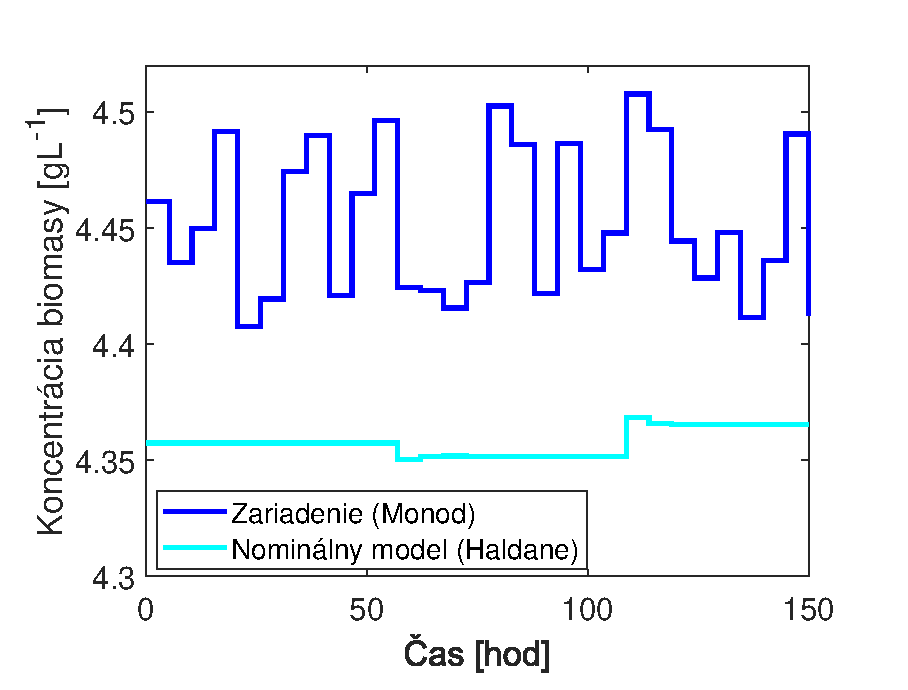
\includegraphics[width=\linewidth]{images/FIR_bio_data}
		\caption{Časový priebeh koncentrácie biomasy.\newline}
		\label{fig:FIR_bio_data}
	\end{subfigure}
	\begin{subfigure}[b]{0.49\textwidth}
		\centering
		\includegraphics[width=\linewidth]{images/FIR_bio_ident}
		\caption{Porovnanie nameraných údajov a výstupov z FIR modelu.}
		\label{fig:FIR_bio_ident}
	\end{subfigure}
\caption{Identifikácia FIR modelu metódou garantovaného odhadu parametrov v tretej iterácii. Zobrazené sú namerané údaje (čierna), výstup FIR modelu identifikovaného MNŠ (zelená) a garantovaná oblasť výstupov FIR modelov, ktorá je definovaná minimálnou (červená) a maximálnou (modrá) realizáciou modelu.}
\label{fig:FIR_bio_identification}
\end{figure}

Výsledok určenia minimálneho rádu FIR modelu v tretej iterácii pomocou GOP bol podobný ako v predchádzajúcich iteráciách. Najjednoduchší model, ktorý dokáže tieto dáta opísať, v rámci stanovenej chyby modelu ($ \delta_{x}=\pm0.1\si{\gram\per\liter} $), je model prvého rádu.
Na rozdiel od prvej iterácie, teraz je už nutné vyhodnotiť kvalitu tohto modelu a porovnať ju s modelmi vyššieho rádu. Na tento účel využijeme Pareto front, ktorý môžeme vidieť na Obr. \ref{fig:FIR_bio_pareto}. Tento graf vyhodnocuje dve vlastnosti modelov a to presnosť modelu, teda vzdialenosť odhadovanej hodnoty od nameranej, a maximálny rozptyl odhadu, ktorý vyjadruje maximálnu vzdialenosť medzi minimálnou resp. maximálnou realizáciou dátového modelu a odhadovanej hodnoty. Tieto vlastnosti sme vyhodnotili pre sto rôznych realizácii šumu merania a spriemerovali. Výsledné hodnoty sú vztiahnuté na model 3. rádu. Čísla pod jednotlivými ukazovateľmi predstavujú FIR model daného rádu. Z Pareto frontu môžeme usúdiť nasledovné. Ak by sme chceli zlepšiť presnosť odhadu zmenou rádu modelu, napr. by sme si zvolili model 2. rádu, získali by sme tým zhoršenie v rozptyle odhadu, ktoré by v tomto prípade bolo kvantitatívne menšie ako zlepšenie v presnosti odhadu. Preto by sa nám oplatilo zvýšiť rád modelu. Na druhej strane by sme sa mali pozrieť aj na absolútne hodnoty týchto vlastností, aby sme vedeli o akom zlepšení resp. zhoršení sa rozprávame. V prípade, že by sme si zvolili namiesto modelu 1. rádu model 5. rádu, dosiahli by sme v priemere zlepšenie presnosti odhadu o 0.0009\si{\gram\per\liter} v absolútnych hodnotách. Takáto hodnota nemá v rámci kvality modelu žiadnu váhu a preto môžeme tvrdiť, že rád modelu vhodný na opis nameraných údajov je FIR model 1. rádu. Tento výsledok vôbec nie je prekvapujúci. Je to spôsobené tým, že vplyv šumu merania je výraznejší ako skutočná zmena v koncentrácii biomasy. Vyššie rády modelov by už mohli opisovať šum merania, čo nie je žiadúca vlastnosť dátových modelov. 

V ďalšom kroku musíme zvoliť veľkosť parametrov resp. parametra, ktorý nám zabezpečí, že finálny výstup z FIR modelu bude čo najbližšie ku skutočnému výstupu. Výsledkom garantovaného odhadu parametrov je aj intervalové určenie hodnôt parametrov, ktoré definujú oblasť všetkých možných riešení v rámci stanovenej chyby modelu. V teoretickej časti sme uviedli, že táto oblasť nám garantuje, že skutočné riešenie sa bude nachádzať vo vnútri tohto ohraničenia. Výsledok identifikácie je zobrazený na Obr. \ref{fig:FIR_bio_ident}. Na tomto obrázku môžeme vidieť tri priebehy výstupov, ktoré zodpovedajú FIR modelu 1. rádu -- výstup garantovaného odhadu parametrov, t.j. minimálna a maximálna realizácia FIR modelu a výstup získaný identifikáciou FIR modelu metódou najmenších štvorcov (MNŠ). Keďže aj výstup FIR modelu získaného metódou najmenších štvorcov sa nachádza vo vnútri tejto oblasti, môžeme ho považovať za vhodný na opis nameraných údajov.
\begin{figure}
	\centering
	\includegraphics[width=0.7\linewidth]{images/FIR_bio_pareto}
	\caption{Pareto front FIR modelov identifikovaných na dátach biomasy. Vlastnosti modelov sú relativizované vzhľadom na model 3. rádu.}
	\label{fig:FIR_bio_pareto}
\end{figure}

V prípade, že by sme identifikovali FIR model na údajoch z rozdielu koncentrácie substrátu zariadenia a nominálneho modelu, prišli by sme k podobnému výsledku. Ale na rozdiel od predchádzajúceho prípadu, potrebujeme na opis nameraných dát v tretej iterácii FIR model 2. rádu, vzhľadom na chybu modelu ($ \delta_{s}=\pm0.05\si{\gram\per\liter} $). Tento rozdiel je spôsobený hneď niekoľkými faktormi. Ako možno vidieť na Obr. \ref{fig:FIR_sub_data}, je tu výrazný rozdiel v kvalite dát -- rozptyl šumu nie je tak veľký, aby prekrýval samotnú dynamiku procesu, ako tomu bolo v predchádzajúcom prípade. Ďalej si treba uvedomiť, že ide o nelineárny proces, ktorý sa snažíme opísať lineárnym modelom. Jediná možnosť, ako sa FIR model dokáže vysporiadať s rozličnou odozvou systému na rovnakú veľkosť vstupnej veličiny, je buď zväčšovaním svojho rádu, alebo zväčšovaním chyby modelu pri identifikácii metódou GOP. 
\begin{figure}
	\centering
	\begin{subfigure}[b]{0.49\textwidth}
		\centering
		\includegraphics[width=\linewidth]{images/FIR_sub_data}
		\caption{Časový priebeh koncentrácie substrátu.\newline}
		\label{fig:FIR_sub_data}
	\end{subfigure}
	\begin{subfigure}[b]{0.49\textwidth}
		\centering
		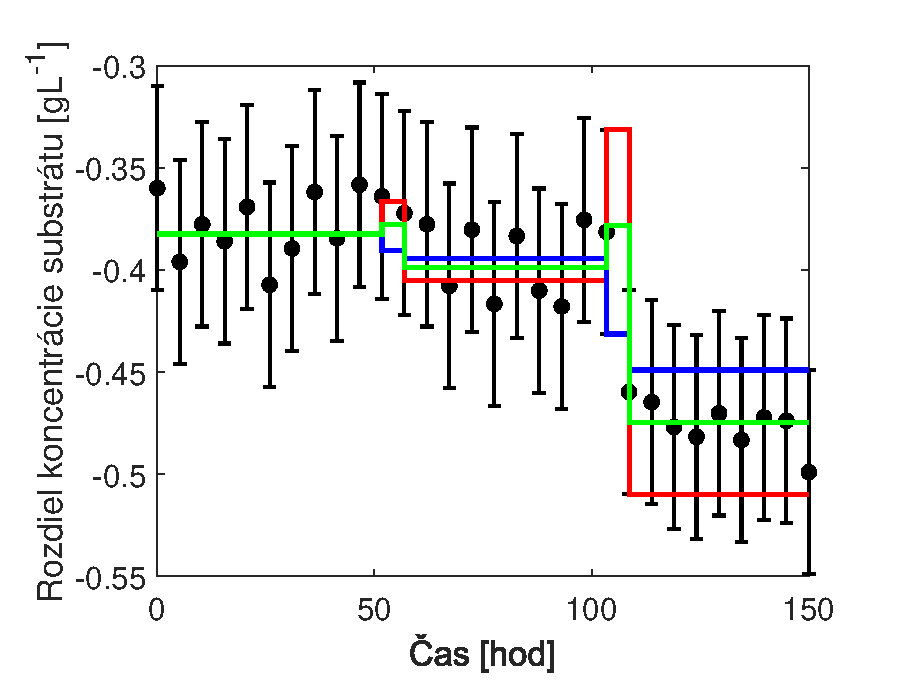
\includegraphics[width=\linewidth]{images/FIR_sub_ident}
		\caption{Porovnanie nameraných údajov a výstupov z FIR modelu.}
		\label{fig:FIR_sub_ident}
	\end{subfigure}
	\caption{Identifikácia FIR modelu metódou garantovaného odhadu parametrov v tretej iterácii. Zobrazené sú namerané údaje (čierna), výstup FIR modelu identifikovaného MNŠ (zelená) a garantovaná oblasť výstupov FIR modelov, ktorá je definovaná minimálnou (červená) a maximálnou (modrá) realizáciou modelu.}
	\label{fig:FIR_sub_identification}
\end{figure}

Relevantnosť rádu modelu posúdime pomocou Pareto frontu, ktorý je zobrazený na Obr. \ref{fig:FIR_sub_ident}. Rád FIR modelov je uvedený pod jednotlivými ukazovateľmi, vlastnosti modelov sme vyhodnotili pre sto realizácii šumu a spriemerovali. Nakoniec sme všetky hodnoty vyjadrili a zobrazili ako násobok veľkosti vlastnosti FIR modelu 3. rádu. Ako si môžeme všimnúť, tento Pareto front ukazuje podobné správanie ako ten z Obr. \ref{fig:FIR_bio_pareto} -- ak by sme chceli zlepšiť presnosť odhadu zvýšením rádu modelu, získali by sme zhoršenie v maximálnom rozptyle odhadu, teda by sa nám rozšíril interval možných hodnôt parametrov. Tak isto by sme mohli uvažovať nad zvýšením radu modelu, pretože zlepšenie v presnosti odhadu je kvantitatívne väčšie ako zhoršenie rozptylu odhadu. Ale táto zmena v presnosti odhadu by vo väčšine prípadov nebola väčšia ako 0.0006\si{\gram\per\liter} v absolútnych hodnotách. Z tohto dôvodu môžeme za vhodný rád modelu označiť FIR model 2. rádu. 
\begin{figure}
	\centering
	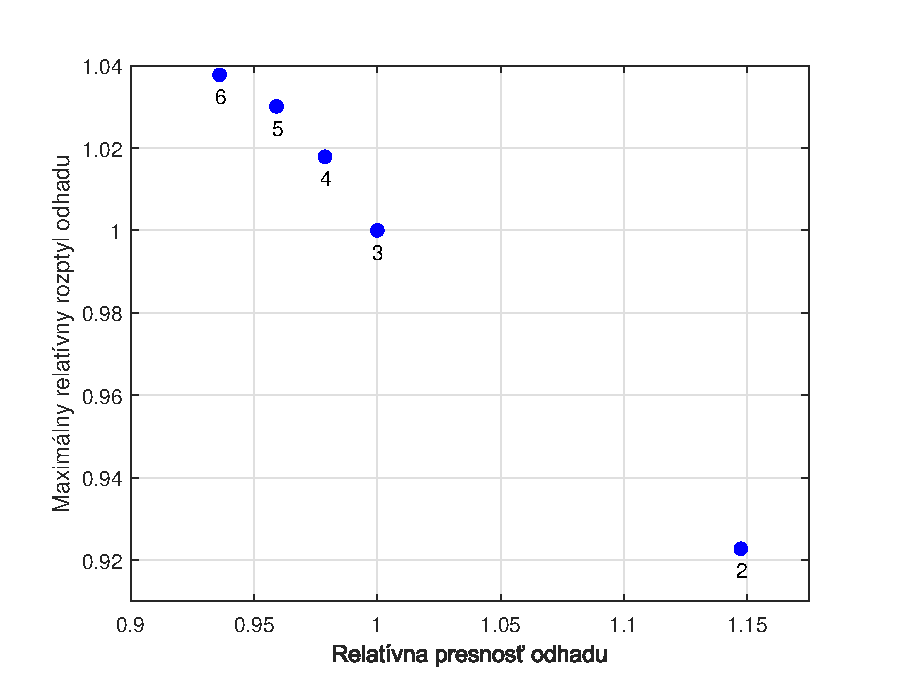
\includegraphics[width=0.7\linewidth]{images/FIR_sub_pareto}
	\caption{Pareto front FIR modelov identifikovaných na dátach substrátu. Údaje o modeloch sú relativizované vzhľadom na model 3. rádu.}
	\label{fig:FIR_sub_pareto}
\end{figure}

Výstupy garantovaného odhadu parametrov FIR modelu môžeme vidieť na Obr. \ref{fig:FIR_sub_ident}. Tak ako v predchádzajúcom prípade sú na obrázku zobrazené výstupy FIR modelu 2. rádu, ktoré zodpovedajú minimálnej a maximálnej realizácii modelu a modelu identifikovaného pomocou metódy najmenších štvorcov. FIR model identifikovaný MNŠ sa opäť nachádza vo vnútri garantovanej oblasti a preto ho môžeme považovať za vhodný na opis nameraných údajov.

Mali by sme spomenúť, že pri voľbe dátových modelov sa až tak nesústredíme na samotný opis dynamiky ako na predikciu ustáleného stavu. Pretože tú potrebujeme na úpravu ustálených stavov nominálneho modelu v účelovej funkcii, ktorú dynamika dátového modelu nezmení. Z tohto dôvodu sa nebudeme až tak dopodrobna zaoberať identifikáciou ARX modelu, ktorý na jednej strane dokáže výrazne lepšie a v kompaktnejšej forme opísať dynamiku procesov, ale na druhej strane predikcia ustálených stavov sa takmer nelíši od FIR modelu. Avšak, z didaktických účelov si ukážeme výsledok identifikácie ARX modelu v tretej iterácii optimalizačného procesu ale iba na dátach substrátu. Tie sú jednak informačne výdatnejšie a pri reálnych zariadeniach sa väčšinou meria iba táto veličina (kvôli už spomínaným problémom s meraním koncentrácie biomasy).

Najjednoduchší ARX model, ktorým vieme opísať rozdiel priebehov nameranej koncentrácie substrátu zariadenia a vygenerovanej koncentrácie substrátu nominálneho modelu z Obr. \ref{fig:ARX_sub_data}, predstavoval diferenčnú rovnicu systému prvého rádu, t.j. polynóm 1. stupňa v čitateli aj menovateli. Výsledok identifikácie metódou garantovaného odhadu parametrov ARX modelu spolu s nameranými údajmi môžeme vidieť na Obr. \ref{fig:ARX_sub_ident}. Dynamika ARX modelu je výrazne komplexnejšia v porovnaní s FIR modelom a pravdepodobne lepšie opisuje skutočnosť ako FIR model, ale ako sme už uviedli, odhad ustálených stavov je porovnateľný.  
\begin{figure}
\centering
	\begin{subfigure}[b]{0.49\textwidth}
		\centering
		\includegraphics[width=\linewidth]{images/ARX_sub_data}
		\caption{Časový priebeh koncentrácie substrátu.\newline}
		\label{fig:ARX_sub_data}
	\end{subfigure}
	\begin{subfigure}[b]{0.49\textwidth}
		\centering
		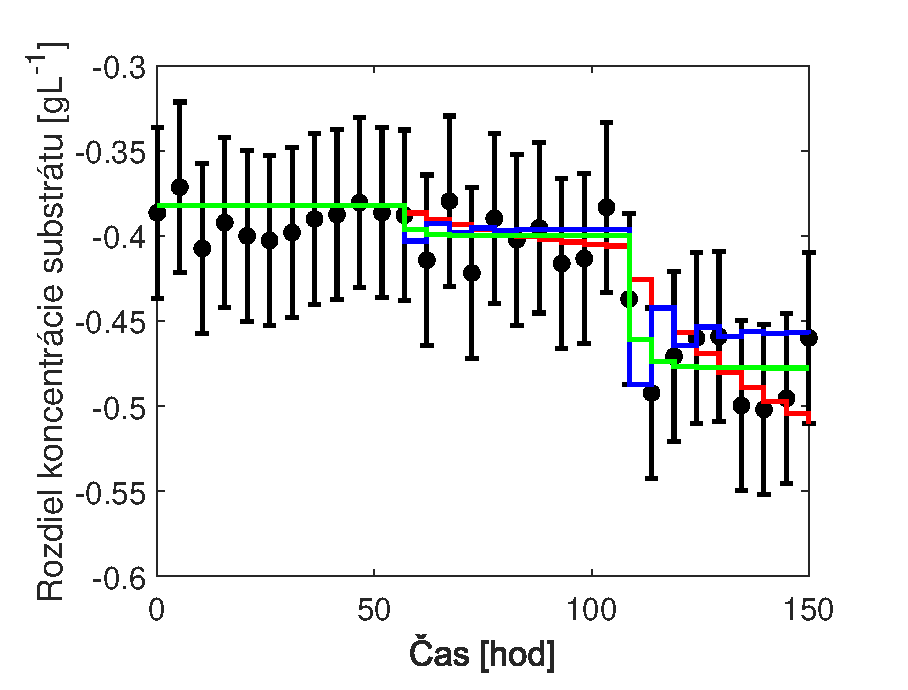
\includegraphics[width=\linewidth]{images/ARX_sub_ident}
		\caption{Porovnanie nameraných údajov a výstupov ARX modelu.}
		\label{fig:ARX_sub_ident}
	\end{subfigure}
\caption{Identifikácia ARX modelu metódou garantovaného odhadu parametrov v tretej iterácii. Zobrazené sú namerané údaje (čierna), výstup ARX modelu identifikovaného MNŠ (zelená) a garantovaná oblasť výstupov ARX modelov, ktorá je definovaná minimálnou (červená) a maximálnou (modrá) realizáciou modelu.}
\label{fig:ARX_sub_identification}
\end{figure}

Problematiku identifikácie dátových modelov, pomocou metódy garantovaného odhadu parametrov, by sme mohli zhrnúť nasledovne. Zatiaľ čo väčšina metód nerieši problematiku voľby rádu modelu, ktorá je dôležitou súčasťou identifikácie dátových modelov a výrazne komplikovanejšou úlohou než odhad parametrov modelov, GOP nám ponúka informácie o minimálnom ráde modelu. V spojení s Pareto frontom dokážeme posúdiť aj kvalitu modelov vyššieho rádu a na základe výsledkov môžeme určiť vhodný rád modelu. V ďalšej časti identifikácie pomocou GOP získavame oblasť všetkých možných riešení, v rámci stanovenej chyby modelu. Táto oblasť, ktorá je určená minimálnou a maximálnou realizáciou modelov, nám zaručuje, že skutočné riešenie leží vo vnútri. Našim cieľom by mala byť snaha o zmenšenie tejto oblasti na čo najmenšiu možnú hodnotu (sme však limitovaný chybou merania), čím si zaručíme presnejší výsledok. To dokážeme spraviť voľbou rádu modelu (maximálny rozptyl odhadu) a chyby modelu.

Ukázali sme, že dokážeme nájsť vhodné dátové modely, či už FIR alebo ARX, na opis údajov, ktoré vyjadrujú rozdiel koncentrácie biomasy alebo substrátu medzi skutočným zariadením (Monod model) a nominálnym modelom (Haldane model). Dynamika týchto modelov bola odlišná, ale v predikcii ustálených stavov boli FIR aj ARX model rovnako dobré. Z tohto dôvodu sme sa rozhodli, že pri konštrukcii hybridných modelov budeme používať výlučne FIR modely. V prípade, že by sme sa zoberali riadením pomocou hybridných modelov, stálo by za zváženie, či radšej neuprednostniť ARX model, ale to by mohlo byť cieľom ďalšieho výskumu.